\documentclass{article}
\usepackage{graphicx} % Required for inserting images
\usepackage{tikz}
\usetikzlibrary{calc}  % para operações de coordenadas
\usetikzlibrary{trees}
\usepackage{minted}
\usepackage{forest}

\forestset{
  null/.style={draw, circle, fill=gray!20, inner sep=1pt, minimum size=0.7cm},
  mynode/.style={draw, circle, minimum size=0.7cm, inner sep=1pt}
}

\begin{document}

\section{Criando vetores}

\begin{center}
  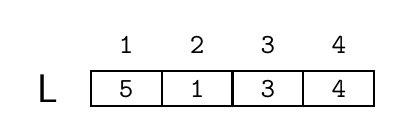
\begin{tikzpicture}

    % Definição de tamanho dos blocos (altura e largura)
    \def\szh{.45cm}
    \def\szw{.9cm}

    % Estilo de bloco retangular
    \tikzstyle{block} = [
      draw, fill=white, rectangle, thick,
      minimum height=\szh, minimum width=\szw
    ];

    % Lista de elementos a serem desenhados nos blocos
    \def\B{5,1,3,4}

    % Desenha a letra 'a' antes dos blocos
    \node at (0,0) {\Large \sf L};

    % Contador para posicionamento dos blocos
    \newcounter{ind}
    \setcounter{ind}{0}

    % Loop para desenhar cada bloco com o elemento correspondente
    \foreach
  \item in \B
    {
      \addtocounter{ind}{1}

      \node[block] at (\theind*\szw+.1cm,0) {\tt
    \item };
      % Números acima dos blocos (índices)

      \node at ({\theind*\szw+.1cm},\szh+.1cm) {\tt \theind};
    }
  \end{tikzpicture}
\end{center}

\section{Criando vetores colorido}

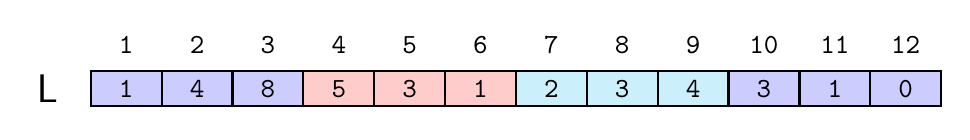
\begin{tikzpicture}
  %--------------------------------------------
  % Definição de tamanho dos blocos
  %--------------------------------------------
  \def\szh{.45cm}   % altura mínima de cada bloco
  \def\szw{.9cm}    % largura mínima de cada bloco

  %--------------------------------------------
  % Estilo de bloco retangular
  %--------------------------------------------
  \tikzstyle{block} = [
    draw, fill=white, rectangle, thick,       % contorno grosso e preenchimento branco
    minimum height=\szh, minimum width=\szw   % tamanho mínimo
  ]

  %--------------------------------------------
  % Lista de valores da sequência
  %--------------------------------------------
  \def\L{1,4,8,5,3,1,2,3,4,3,1,0}

  %--------------------------------------------
  % Rótulo inicial da lista
  %--------------------------------------------
  \node at (0,0) {\Large \sf L};   % letra L na posição inicial

  %--------------------------------------------
  % Loop para desenhar cada bloco colorido com índice
  %--------------------------------------------
  % count=\i cria um contador automático que começa em 1
  \foreach [count=\i]
\item/\cor in {1/blue!20,4/blue!20,8/blue!20,5/red!20,3/red!20,1/red!20,
  2/cyan!20,3/cyan!20,4/cyan!20,3/blue!20,1/blue!20,0/blue!20}
  {
    %----------------------------------------
    % Desenha o bloco preenchido com a cor especificada
    %----------------------------------------
    \node[block, fill=\cor] at ({\i*\szw+.1cm},0) {\tt
  \item};

    %----------------------------------------
    % Exibe o índice do bloco acima
    %----------------------------------------
    \node at ({\i*\szw+.1cm},\szh+.1cm) {\tt \i};
  }
\end{tikzpicture}

\section{Lista Encadeada}

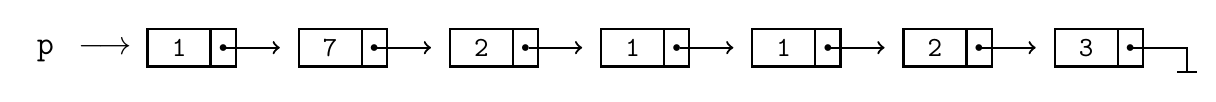
\begin{tikzpicture}

  %--------------------------------------------
  % Escala geral (deixa o diagrama mais compacto)
  %--------------------------------------------
  \begin{scope}[xscale=.8, yscale=.8]

    %--------------------------------------------
    % Rótulo inicial do ponteiro p
    %--------------------------------------------
    \node at (-1, .25) {\tt \large p\: $\longrightarrow$};

    %--------------------------------------------
    % Laço para desenhar os nós intermediários da lista
    % Cada par (x/y) indica:
    %   x -> posição (índice do nó)
    %   y -> valor armazenado
    %--------------------------------------------
    \foreach \x/\y in {0/1, 1/7, 2/2, 3/1, 4/1, 5/2}
    {
      % Desenha o nó:
      % - Cada nó é composto por dois retângulos lado a lado
      %   (um para o valor, outro para o ponteiro)
      \draw[thick]
      (2.4*\x + 0, 0) rectangle (2.4*\x + 1.0, .6)  % campo de dado
      (2.4*\x + 1.0, 0) rectangle (2.4*\x + 1.4, .6); % campo de ponteiro

      % Desenha a seta que sai do ponteiro para o próximo nó
      \draw[->, thick]
      (2.4*\x + 1.25, .3) -- (2.4*\x + 2.1, .3);

      % Valor do nó no campo de dado
      \node at (2.4*\x + 0.5, .30) {\tt \y};

      % Ponto indicando o ponteiro (representação simbólica)
      \node at (2.4*\x + 1.2, .30) {\tiny $\bullet$};
    }

    %--------------------------------------------
    % Último nó da lista (ponteiro nulo)
    %--------------------------------------------
    \def\x{6}  % posição do último nó
    \def\y{3}  % valor armazenado

    % Nó final
    \draw[thick]
    (2.4*\x + 0, 0) rectangle (2.4*\x + 1.0, .6)
    (2.4*\x + 1.0, 0) rectangle (2.4*\x + 1.4, .6);

    % Seta com final em T (|-), representando NULL
    \draw[-|, thick]
    (2.4*\x + 1.25, .3) -- (2.4*\x + 2.1, .3) -- (2.4*\x + 2.1, -.1);

    % Valor do último nó
    \node at (2.4*\x + 0.5, .30) {\tt \y};

    % Ponto do ponteiro
    \node at (2.4*\x + 1.2, .30) {\tiny $\bullet$};

  \end{scope}

\end{tikzpicture}

\section{Árvore Binária}

% Desenho de uma árvore binária manualmente
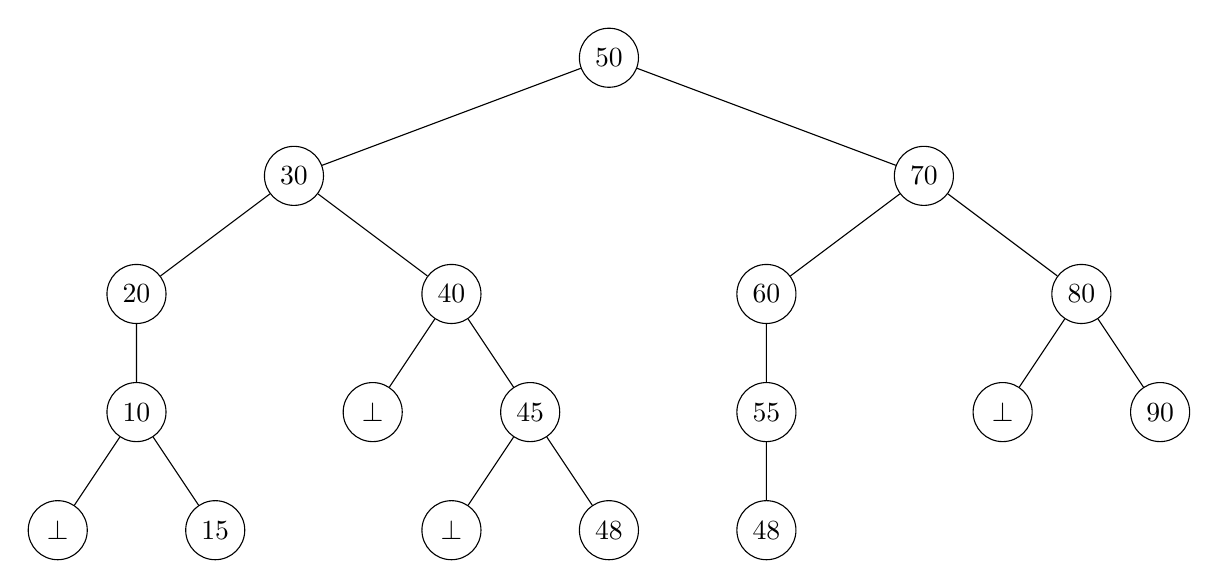
\begin{tikzpicture}[
    % Distância vertical entre níveis
    level distance=1.5cm,
    % Distâncias horizontais entre filhos em cada nível
    level 1/.style={sibling distance=8cm},
    level 2/.style={sibling distance=4cm},
    level 3/.style={sibling distance=2cm},
    % Estilo padrão dos nós
    every node/.style={circle, draw, minimum size=0.75cm}
  ]

  % Nó raiz com valor 50
  \node {50}
  % Filho esquerdo
  child {
    node {30}
    % Subárvore esquerda de 30
    child {
      node {20}
      child {
        node {10}
        % Folha esquerda (nó nulo)
        child { node {$\bot$} }
        % Folha direita (nó 15)
        child { node {15} }
      }
    }
    % Subárvore direita de 30
    child {
      node {40}
      child { node {$\bot$} }
      child {
        node {45}
        child { node {$\bot$} }
        child { node {48} }
      }
    }
  }
  % Filho direito
  child {
    node {70}
    child {
      node {60}
      child {
        node {55}
        child { node {48} }
      }
    }
    child {
      node {80}
      child { node {$\bot$} }
      child { node {90} }
    }
  };

\end{tikzpicture}

% \begin{center}
% \begin{forest}
%   % Configuração global da árvore
%   for tree={
%     grow'=south,        % A árvore cresce de cima para baixo
%     edge={thick},       % Arestas mais grossas
%     s sep=16mm,          % Espaçamento horizontal entre irmãos
%     l sep=12mm,          % Espaçamento vertical entre níveis
%     anchor=center      % Centraliza cada nó na linha
%   }

%   % ======= Estrutura da árvore binária =======
%   [50, mynode % nó raiz
%     [30, mynode % filho esquerdo
%       [20, mynode % filho esquerdo de 30
%         [10, mynode % filho esquerdo de 20
%           [$\emptyset$, null]      % filho esquerdo de 10 (nó nulo, desenhado em cinza)
%           [15, mynode]     % filho direito de 10 (nó normal)
%         ]
%       ]
%       [40, mynode % filho direito de 30
%         [$\emptyset$, null]        % filho esquerdo de 40 (nó nulo)
%         [45, mynode              % filho direito de 40
%           [$\emptyset$, null]      % filho esquerdo de 45 (nó nulo)
%           [48, mynode]     % filho direito de 45 (nó normal)
%         ]
%       ]
%     ]
%     [70, mynode % filho direito de 50
%       [60, mynode % filho esquerdo de 70
%         [55, mynode
%           [48, mynode]     % filho esquerdo de 55
%           [$\emptyset$, null]      % filho direito de 55
%         ]
%       ]
%       [80, mynode % filho direito de 70
%         [$\emptyset$, null]        % filho esquerdo de 80
%         [90, mynode]       % filho direito de 80
%       ]
%     ]
%   ]
% \end{forest}

% \end{center}

\section{Exercícios}

Suponha que a estrutura node\_tree tem um novo campo num\_folhas. Inicialmente, você tem uma árvore onde os nós estão todos com o num\_folhas igual a -1.

\begin{minted}{C++}
typedef struct node_tree{
    int chave;
    int valor;
    int num_folhas;
    struct node_tree * esq;
    struct node_tree * dir;
} node_tree;
\end{minted}

Escreva uma função void preenche\_num\_folhas(Arvore* arv) que recebe uma árvore e preenche o campo num\_folhas de todos os nós da árvore.

% Duas árvores lado a lado usando minipage
\begin{minipage}{0.5\textwidth} % Primeira minipage (50% da largura do texto)
  \centering
  \subsection*{Entrada}
  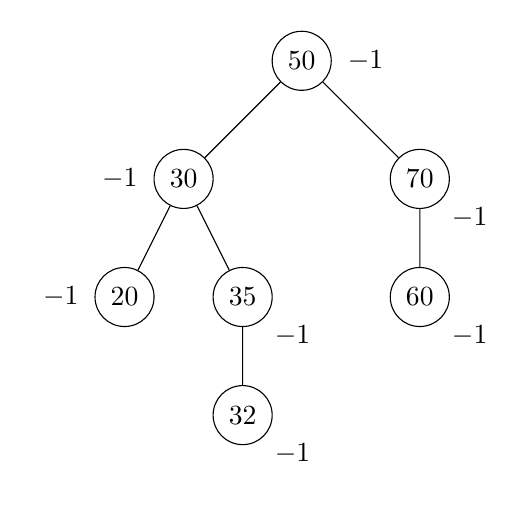
\begin{tikzpicture}[
      level distance=1.5cm,
      level 1/.style={sibling distance=3cm},
      level 2/.style={sibling distance=1.5cm},
      every node/.style={circle, draw, minimum size=0.75cm}
    ]
    % Primeira árvore
    \node[label=360:$-1$] {50}
    child {
      node[label=180:$-1$] {30}
      child { node[label=180:$-1$] {20}   }
      child { node[label=330:$-1$] {35}
        child {
          node[label=330:$-1$] {32}
        }
      }
    }
    child {
      node[label=330:$-1$] {70}
      child { node[label=330:$-1$] {60} }
    };
  \end{tikzpicture}

\end{minipage}%
\begin{minipage}{0.5\textwidth} % Segunda minipage (50% da largura do texto)
  \centering
  \subsection*{Saída}
  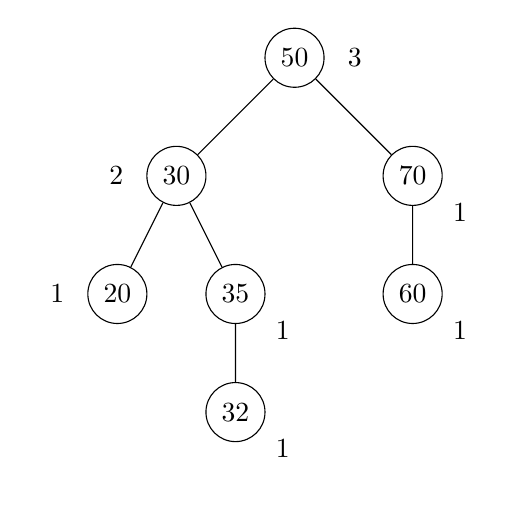
\begin{tikzpicture}[
      level distance=1.5cm,
      level 1/.style={sibling distance=3cm},
      level 2/.style={sibling distance=1.5cm},
      every node/.style={circle, draw, minimum size=0.75cm}
    ]
    % Primeira árvore
    \node[label=360:$3$] {50}
    child {
      node[label=180:$2$] {30}
      child { node[label=180:$1$] {20}   }
      child { node[label=330:$1$] {35}
        child {
          node[label=330:$1$] {32}
        }
      }
    }
    child {
      node[label=330:$1$] {70}
      child { node[label=330:$1$] {60} }
    };
  \end{tikzpicture}
\end{minipage}

Suponha que a estrutura {\tt node\_tree} tem um novo campo {\tt mais\_esquerda} e {\tt mais\_direita}. Inicialmente, você tem uma árvore onde os nós estão todos com o campo mais\_esquerda e mais\_direita apontado para NULL

\begin{minted}{C++}
typedef struct node_tree{
    int chave;
    int valor;
    struct node_tree * mais_esquerda;
    struct node_tree * mais_direita;
    struct node_tree * esq;
    struct node_tree * dir;
} node_tree;

typedef struct Arvore{
  node_tree * raiz;
} Arvore;
\end{minted}

Escreva uma função {\tt void preenche\_arvore(Arvore* arv)} que recebe uma árvore e preenche o campo {\tt mais\_esquerda} e {\tt mais\_direita} de todos os nós da árvore.

% Duas árvores lado a lado usando minipage
\begin{minipage}{0.5\textwidth} % Primeira minipage (50% da largura do texto)
  \centering
  \subsection*{Entrada}
  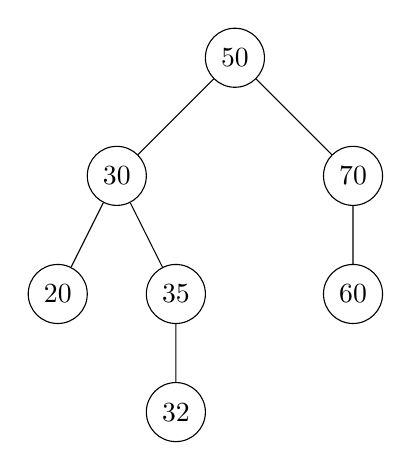
\begin{tikzpicture}[
      level distance=1.5cm,
      level 1/.style={sibling distance=3cm},
      level 2/.style={sibling distance=1.5cm},
      every node/.style={circle, draw, minimum size=0.75cm}
    ]
    % Primeira árvore
    \node {50}
    child {
      node {30}
      child { node {20}   }
      child { node {35}
        child {
          node {32}
        }
      }
    }
    child {
      node {70}
      child { node {60} }
    };
  \end{tikzpicture}

\end{minipage}%
\begin{minipage}{0.5\textwidth} % Segunda minipage (50% da largura do texto)
  \centering
  \subsection*{Saída}
  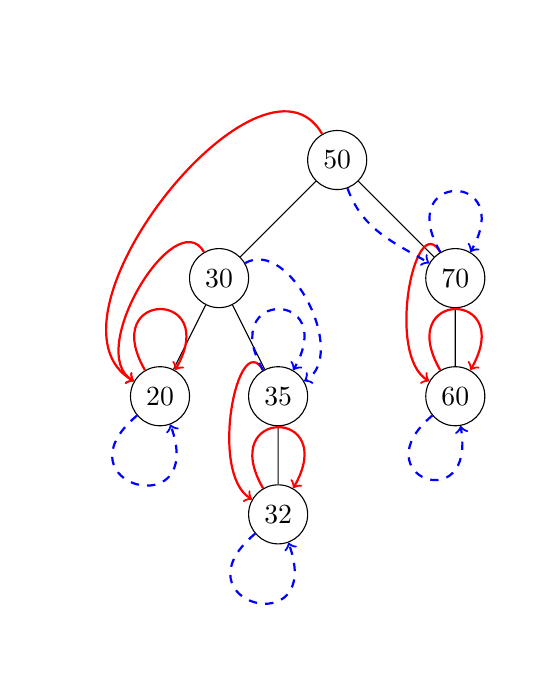
\begin{tikzpicture}[
      level distance=1.5cm,
      level 1/.style={sibling distance=3cm},
      level 2/.style={sibling distance=1.5cm},
      every node/.style={circle, draw, minimum size=0.75cm}
    ]
    % Primeira árvore
    \node (n50) {50}
    child {
      node (n30) {30}
      child { node (n20) {20}   }
      child { node (n35) {35}
        child {
          node (n32) {32}
        }
      }
    }
    child {
      node (n70) {70}
      child { node (n60) {60} }
    };

    \draw[->, red, thick] (n30) to[out=120, in=150] (n20);
    \draw[->, red, thick] (n20) to[out=120, in=60, looseness=8] (n20);
    \draw[->, red, thick] (n32) to[out=120, in=60, looseness=8] (n32);
    \draw[->, red, thick] (n35) to[out=120, in=150] (n32);
    \draw[->, red, thick] (n50) to[out=120, in=150] (n20);
    \draw[->, red, thick] (n70) to[out=120, in=150] (n60);
    \draw[->, red, thick] (n60) to[out=120, in=60, looseness=8] (n60);

    \draw[->, blue, thick, dashed] (n35) to[out=120, in=60, looseness=8] (n35);
    \draw[->, blue, thick, dashed] (n32) to[out=220, in=290, looseness=8] (n32);
    \draw[->, blue, thick, dashed] (n20) to[out=220, in=290, looseness=8] (n20);
    \draw[->, blue, thick, dashed] (n30) to[out=30, in=30] (n35);
    \draw[->, blue, thick, dashed] (n50) to[out=290, in=150] (n70);
    \draw[->, blue, thick, dashed] (n70) to[out=120, in=60, looseness=8] (n70);
    \draw[->, blue, thick, dashed] (n60) to[out=220, in=280, looseness=8] (n60);

  \end{tikzpicture}
\end{minipage}

\end{document}
